\documentclass[a4paper]{article} 
\addtolength{\hoffset}{-2.25cm}
\addtolength{\textwidth}{4.5cm}
\addtolength{\voffset}{-3.25cm}
\addtolength{\textheight}{5cm}
\setlength{\parskip}{0pt}
\setlength{\parindent}{0in}

%----------------------------------------------------------------------------------------
%	PACKAGES AND OTHER DOCUMENT CONFIGURATIONS
%----------------------------------------------------------------------------------------

\usepackage[italicdiff]{physics}
%\usepackage{derivative}
\usepackage{tasks}
\usepackage{blindtext} % Package to generate dummy text
\usepackage{charter} % Use the Charter font
\usepackage[utf8]{inputenc} % Use UTF-8 encoding
\usepackage{microtype} % Slightly tweak font spacing for aesthetics
\usepackage[T1]{fontenc}
\usepackage{polski}
\usepackage{enumerate}
\usepackage[utf8]{inputenc}
\usepackage[english, ngerman]{babel} % Language hyphenation and typographical rules
\usepackage{amsthm, amsmath, amssymb} % Mathematical typesetting
\usepackage{float} % Improved interface for floating objects
\usepackage[final, colorlinks = true, 
            linkcolor = black, 
            citecolor = black]{hyperref} % For hyperlinks in the PDF
\usepackage{graphicx, multicol} % Enhanced support for graphics
\usepackage{xcolor} % Driver-independent color extensions
\usepackage{marvosym, wasysym} % More symbols
\usepackage{rotating} % Rotation tools
\usepackage{censor} % Facilities for controlling restricted text
\usepackage{listings, style/lstlisting} % Environment for non-formatted code, !uses style file!
\usepackage{pseudocode} % Environment for specifying algorithms in a natural way
\usepackage{style/avm} % Environment for f-structures, !uses style file!
\usepackage{booktabs} % Enhances quality of tables
\usepackage{tikz-qtree} % Easy tree drawing tool
\tikzset{every tree node/.style={align=center,anchor=north},
         level distance=2cm} % Configuration for q-trees
\usepackage{style/btree} % Configuration for b-trees and b+-trees, !uses style file!
\usepackage[backend=biber,style=numeric,
            sorting=nyt]{biblatex} % Complete reimplementation of bibliographic facilities
\addbibresource{ecl.bib}
\usepackage{csquotes} % Context sensitive quotation facilities
\usepackage[yyyymmdd]{datetime} % Uses YEAR-MONTH-DAY format for dates
\renewcommand{\dateseparator}{-} % Sets dateseparator to '-'
\usepackage{fancyhdr} % Headers and footers
\pagestyle{fancy} % All pages have headers and footers
\fancyhead{}\renewcommand{\headrulewidth}{0pt} % Blank out the default header
\fancyfoot[L]{} % Custom footer text
\fancyfoot[C]{} % Custom footer text
\fancyfoot[R]{\thepage} % Custom footer text
\newcommand{\note}[1]{\marginpar{\scriptsize \textcolor{red}{#1}}} %
\graphicspath{ {./images/} }

%----------------------------------------------------------------------------------------

\begin{document}

%-------------------------------
%	TITLE SECTION
%-------------------------------

\fancyhead[C]{}
\hrule \medskip % Upper rule
\begin{minipage}{0.295\textwidth} 
\raggedright
\footnotesize
Antoni Dąbrowski \hfill\\   
Nr. indeksu 317214\hfill\\
Mail: 317214@uwr.edu.pl
\end{minipage}
\begin{minipage}{0.4\textwidth} 
\centering 
\large 
Statystyka\\ 
\normalsize 
Laboratorium - lista I\\ 
\end{minipage}
\begin{minipage}{0.295\textwidth} 
\raggedleft
\today\hfill\\
\end{minipage}
\medskip\hrule 
\bigskip

%-------------------------------
%	CONTENTS
%-------------------------------


\section{Zadanie pierwsze}
Wygeneruj n obserwacji z rozkładu $N(\theta,\sigma^2)$.
\begin{itemize}
	\item $n=50$, $\theta=1$, $\sigma=1$,
	\item $n=50$, $\theta=4$, $\sigma=1$,
	\item $n=50$, $\theta=1$, $\sigma=2$.
\end{itemize}
Na tej podstawie oblicz wartości estymatora parametru $\Theta$ postaci
\begin{itemize}
\item $\hat{\theta}_1 = \bar{X} = (1/n)\sum_{i=1}^nX_i$,
\item $\hat{\theta}_2 = Me\{X_1,...,X_n\},$
\item $\hat{\theta}_3 = \sum_{i=1}^nw_iX_i,\sum_{i=1}^n=1,0\leq w_i\leq 1,i=1,...,n,$ z własnym wyborem wag
\item $\hat{\theta}_4 = \sum_{i=1}^nw_iX_{i:n}, gdzie X_{1:n}\leq\hdots\leq X_{n:n}$ są uporządkowanymi obserwacjami $X_1,...,X_n$,$$w_i=\phi(\Phi^{-1}(\frac{i-1}{n}))-\phi(\Phi^{-1}(\frac{i}{n})),$$ przy czym $\phi$ jest gęstością, a $\Phi$ dystrybuantą standardowego rozkładu normalnego $N(0,1)$.
\end{itemize}
Doświadczenie powtórz $10 000$ razy. Na tej podstawie oszacuj wariancję, błąd średniokwadratowy oraz obciążenie każdego z estymatorów. Przedyskutuj uzyskane wyniki.

\subsection{Rozwiązanie}
Użyte wzory:
\begin{itemize}
\item wariancja $1/n\sum_{i=1}^n(\bar{X}-X_i)^2$
\item błąd średniokwadratowy $1/n\sum_{i=1}^n(\theta-X_i)^2$
\item obciążenie estymatora $|\theta - \bar{X}|$
\end{itemize}

\begin{table}[H]
\centering
\begin{tabular}{|c|c|c|c|}
\hline
\multicolumn{4}{|c|}{$n=50$, $\theta=1$, $\sigma=1$} \\ \hline
                  & \textbf{wariancja}   & \textbf{błąd średniokwadratowy} & \textbf{obciążenie estymatora} \\ \hline
$\hat{\theta}_1$ & 0.02020486 & 0.02020939 & 0.00212849 \\ \hline
$\hat{\theta}_2$ & 0.03103397 & 0.03103752 & 0.00188406 \\ \hline
$\hat{\theta}_3$ & 0.02673854 & 0.02674088 & 0.00152817 \\ \hline
$\hat{\theta}_4$ & 0.00952659 & 0.01035948 & 0.02885990 \\ \hline
\end{tabular}
\end{table}


\begin{table}[H]
\centering
\begin{tabular}{|c|c|c|c|}
\hline
\multicolumn{4}{|c|}{$n=50$, $\theta=4$, $\sigma=1$} \\ \hline
                  & \textbf{wariancja}   & \textbf{błąd średniokwadratowy} & \textbf{obciążenie estymatora} \\ \hline
$\hat{\theta}_1$ & 0.02012309 & 0.02012547 & 0.00154499 \\ \hline
$\hat{\theta}_2$ & 0.03048605 & 0.03048676 & 0.00084350 \\ \hline
$\hat{\theta}_3$ & 0.02660123 & 0.02661033 & 0.00301660 \\ \hline
$\hat{\theta}_4$ & 0.00981973 & 9.18248034 & 3.02864006 \\ \hline
\end{tabular}
\end{table}

\begin{table}[H]
\centering
\begin{tabular}{|c|c|c|c|}
\hline
\multicolumn{4}{|c|}{$n=50$, $\theta=1$, $\sigma=2$} \\ \hline
                  & \textbf{wariancja}   & \textbf{błąd średniokwadratowy} & \textbf{obciążenie estymatora} \\ \hline
$\hat{\theta}_1$ & 0.07943470 & 0.07944444 & 0.00312149 \\ \hline
$\hat{\theta}_2$ & 0.12105089 & 0.12105846 & 0.00275068 \\ \hline
$\hat{\theta}_3$ & 0.10503579 & 0.10504052 & 0.00217525 \\ \hline
$\hat{\theta}_4$ & 0.03794412 & 0.92673064 & 0.94275474 \\ \hline
\end{tabular}
\end{table}

Wnioskując z obserwacji wyników eksperymentu pierwsze trzy estymatory są nieobciążone. Operator $\hat{\theta}_4$ ma wyraźnie większe obciążenie oraz błąd średniokwadratowy od  pozostałych, za to przy jego zastosowaniu uzyskałem najmniejszą wariancję wyniku.

\section{Zadanie drugie}
Omów komendę \textbf{set.seed(1)} oraz jej potencjalne zastosowania.

\subsection{Rozwiązanie}
Komenda inicjalizuje generator liczb losowych w sposób powtarzalny. Pozwala to wielokrotnie wykonywać eksperyment dla tych samych losowych danych wejściowych. Jest to niezwykle przydatna funkcja. Wielokrotnie używałem jej do analizy przypadków marginalnych. Zdażało mi się tak, że mój program opierający się na losowości czasem zachowywał się w inny sposób niż bym tego oczekiwał, w takim przypadku funkcja \textbf{seed} pozwalała mi wielokrotnie wrócić do danego ''błędnego''  ustawienia i je przeanalizować.


\section{Zadanie trzecie}
Omów konieczność numerycznego wyznaczania estymatorów największej wiarogodności na przykładzie estymacji parametru przesunięcia w rozkładzie logistycznym.

\subsection{Rozwiązanie}
Aby wyznaczyć estymator największej wiarygodności chcemy znaleźć taki parametr, który maksymalizuje funkcję wiarygodności. W przypadku rozkładu logistycznego pokazaliśmy, że funkcja taka osiąga maksimum i to w tylko jednym punkcie. Zatem mamy pewność, że istnieje MLE tego rozkładu, jednakże nie mamy zwartego równania pozwalającego wyznaczyć szukaną wartość. Stąd wynika konieczność zastosowania algorytmu numerycznego.

\section{Zadanie czwarte}
Omów wybraną metodę numeryczną pozwalającą na wyznaczenie estymatora największej wiarogodności.

\subsection{Rozwiązanie}
Metoda Newtona - Aby być przekonanym o skuteczności metody funkcja na badanym odcinku  musi być monotoniczna, znak drugiej pochodnej musi być stały oraz musi posiadać tam przynajmniej jedno miejsce zerowe. Idea polega na stopniowym poprawianiu przybliżenia miejsca zerowego. Niech $x_0$ będzie punktem początkowym. Dobrze, aby taki punkt znajdował się możliwie jak najbliżej miejsca zerowego. Wyznaczamy punkt przecięcia prostej stycznej do funkcji w $x_0$ z osią OX. Ten punkt traktujemy jako nowe przybliżenie miejsca zerowego. $$x_{n+1}=x_n - \frac{f(x_n)}{f'(x_n)}$$
Metoda ma sznsę działać również, gdy funkcja nie spełnia warunku wypukłości lub nie jest monotoniczna. Jeśli jednak wciąż nie udaje się uzyskać rezultatów, można zastosować metodę bisekcji o dużo skromniejszych wymaganiach, jednak działającą znacznie wolniej.

\section{Zadanie piąte}
Wygeneruj n obserwacji z rozkładu logistycznego $L(\theta,\sigma)$ z parametrami przesunięcia $\theta$ i skali $\sigma$.
\begin{itemize}
\item $n=50$, $\theta=1$, $\sigma=1$
\item $n=50$, $\theta=4$, $\sigma=1$
\item $n=50$, $\theta=1$, $\sigma=2$
\end{itemize}
Oszacuj wartość estymatora największej wiarygodności parametru $\theta$ na podstawie wygenerowanegj próby. Przedyskutuj wybór punktu początkowego oraz liczbę kroków w algorytmie.\\

Doświadczenie powtórz 10 000 razy. Na tej podstawie oszacuj wariancję, błąd średniokwadratowy oraz obciążenie estymatora. Przedyskutuj uzyskane wyniki.
\subsection{Rozwiązanie}
Funkcja gęstości rozkładu logistycznego:
$$f(x;\theta ,\sigma )=\frac {e^{-(x-\theta )/\sigma}}{\sigma(1+e^{-(x-\theta )/\sigma})^2}$$
Funkcja wiarygodności oraz jej logarytm:
$$L(\theta,\sigma)=\prod_{i=1}^n\frac {e^{-(x_i-\theta )/\sigma}}{\sigma(1+e^{-(x_i-\theta )/\sigma})^2}$$
$$l(\theta,\sigma)=\sum_{i=1}^nlog\frac {e^{-(x_i-\theta )/\sigma}}{s(1+e^{-(x_i-\theta )/\sigma})^2}=\sum_{i=1}^n[\frac{-x_i}{\sigma}+\frac{\theta}{\sigma}-\sigma-2log(1+e^{-(x-\theta )/\sigma})]=\frac{n\theta}{\sigma}-\frac{n\bar{x}}{\sigma}-n\sigma-2\sum_{i=1}^nlog(1+e^{-(x-\theta )/\sigma})$$
Aby wyznaczyć MLE zbadamy przebieg funkcji $l$:
$$\pdv{}{\theta} l(\theta,\sigma)=\frac{n}{\sigma}-2\sum_{i=1}^n\frac{e^{-(x_i-\theta)/\sigma}}{\sigma(1+e^{-(x_i-\theta)/\sigma})}\rightarrow\frac{n}{2\sigma}=\sum_{i=1}^n\frac{e^{-(x_i-\theta)/\sigma}}{\sigma(1+e^{-(x_i-\theta)/\sigma})}$$
$$\pdv{^2}{\theta^2} l(\theta,\sigma)=\sum_{i=1}^n\frac{e^{(x_i-\theta)/\sigma}}{(\sigma e^{(x_i-\theta)/\sigma}+\sigma)^2}$$
Zauważmy, że gdy $\theta\rightarrow\infty$, to $\pdv{}{\theta} l(\theta,\sigma)$ zbiega do $\frac{n}{\sigma}$, natomiast gdy $\theta\rightarrow-\infty$, to $\pdv{}{\theta} l(\theta,\sigma)$ dąży do 0. Ponadto widać, że na całej dziedzinie druga pochodna cząstkowa funkcji l jest dodatnia. Zatem mamy pewność, że możemy znaleźć MLE. Posłóżę się do tego celu metodą Newtona. A za punkt początkowy przyjmę średnią próbki. Algorytm:
$$z_0=\bar{X}, z_{n+1} = z_n - \frac{\pdv{}{\theta}l(z_n,\sigma)}{\pdv{^2}{\theta^2}l(z_n,\sigma)}$$

\begin{table}[H]
\centering
\begin{tabular}{|c|c|c|c|}
\hline
\multicolumn{4}{|c|}{\textbf{Obserwacje}}                                                       \\ \hline
         & wariancja           & błąd średniokwadratowy & obciążenie estymatora \\ \hline
$n=50,\theta=1,\sigma=1$ & 0.05801277 & 0.05801772 & 0.00222632 \\ \hline
$n=50,\theta=4,\sigma=1$  & 0.05881378 & 0.05882692 & 0.00362511 \\ \hline
$n=50,\theta=1,\sigma=2$  & 0.25275808 & 0.25277557 & 0.00418168 \\ \hline
\end{tabular}
\end{table}

Znaleziony wzór skutecznie pozwala estymować szukaną wartość.

\section{Zadanie szóste}
Wygeneruj n obserwacji z rozkładu Cauchy'ego $C(\theta,\sigma)$ z parametrem przesunięcia $\theta$ i skali $\sigma$.
\begin{itemize}
\item $n=50, \theta=1, \sigma=1$
\item $n=50, \theta=4, \sigma=1$
\item $n=50, \theta=1, \sigma=2$
\end{itemize}
Oszacuj wartość estymatora największej wiarygodności parametru $\theta$ na podstawie wygenerowanegj próby. Przedyskutuj wybór punktu początkowego oraz liczbę kroków w algorytmie.\\

Doświadczenie powtórz 10 000 razy. Na tej podstawie oszacuj wariancję, błąd średniokwadratowy oraz obciążenie estymatora. Przedyskutuj uzyskane wyniki.
\subsection{Rozwiązanie}
Funkcja gęstości rozkładu Cauchy'ego:
$$f(x;\theta,\sigma)=\frac{1}{\pi\sigma[1+(\frac{x-\theta}{\sigma})^2]}$$
Funkcja wiarygodności oraz jej logarytm:
$$L(\theta,\sigma)=\prod_{i=1}^n\frac{1}{\pi\sigma[1+(\frac{x-\theta}{\sigma})^2]}$$
$$l(\theta,\sigma)=\sum_{i=1}^nlog\frac{1}{\pi\sigma[1+(\frac{x_i-\theta}{\sigma})^2]}=\sum_{i=1}^n[-log\pi\sigma-log(1+(\frac{x_i-\theta}{\sigma})^2)]=-nlog(\pi\sigma)-\sum_{i=1}^nlog(1+(\frac{x_i-\theta}{\sigma})^2)$$
Aby wyznaczyć MLE zbadamy przebieg funkcji $l$:
$$\pdv{}{\theta}l(\theta,\sigma)=\sum_{i=1}^n\frac{2(\theta-x_i)}{(\theta-x_i)^2+s^2}$$
$$\pdv{^2}{\theta^2}l(\theta,\sigma)=\sum_{i=1}^n-\frac{2(\theta-x_i-\sigma)(\theta-x_i+\sigma)}{((\theta-x_i)^2+\sigma^2)^2}$$
Aby znaleźć maksimum zajmiemy się znalezieniem miejsc zerowych funkcji $\pdv{}{\theta}l(\theta,\sigma)$. Zrobimy to poprzez wykorzystanie metody Newtona. Jednak w tym przypadku bardzo istotne okazuje się dobranie punktu początkowego poszukiwań. Średnia arytetyczna nie jest dobrym estymatorem zmiennych z rozkładu Cauchy'ego, ze względu na wysokie prawdopodobieństwo uzyskania skrajnych wartości. Sensownymi pomysłami wydają się być mediana lub średnia arytmetyczna pewnej frakcji "środkowych" punktów. Wybrałem pierwszy estymator. Algorytm:
$$z_0=Me\{x_1,...,x_n\}, z_{n+1}=z_n - \frac{\pdv{}{\theta}l(z_n,\sigma)}{\pdv{^2}{\theta^2}l(z_n,\sigma)}$$


\begin{table}[H]
\centering
\begin{tabular}{|c|c|c|c|}
\hline
\multicolumn{4}{|c|}{\textbf{Obserwacje}}                                                       \\ \hline
         & wariancja           & błąd średniokwadratowy & obciążenie estymatora \\ \hline
$n=50,\theta=1,\sigma=1$ & 0.04138948 & 0.04139330 & 0.00195417 \\ \hline
$n=50,\theta=4,\sigma=1$ & 0.04213790 & 0.04215631 & 0.00428994 \\ \hline
$n=50,\theta=1,\sigma=2$ & 0.20168464 & 0.20170648 & 0.00467358 \\ \hline
\end{tabular}
\end{table}



\section{Zadanie siódme}
Powtórz eksperyment numeryczny z zadań 1, 5, 6 dla $n=20$ i $n=100$. Przedyskutuj uzyskane rezultaty w nawiązaniu do wcześniejszych wyników.

\subsection{Rozwiązanie}
Zadanie 1:

\begin{table}[H]
\centering
\begin{tabular}{|c|c|c|c|}
\hline
\multicolumn{4}{|c|}{$n=20$, $\theta=1$, $\sigma=1$} \\ \hline
                  & \textbf{wariancja}   & \textbf{błąd średniokwadratowy} & \textbf{obciążenie estymatora} \\ \hline
$\hat{\theta}_1$ & 0.05055495 & 0.05055513 & 0.00042939 \\ \hline
$\hat{\theta}_2$ & 0.07318377 & 0.07318953 & 0.00240106 \\ \hline
$\hat{\theta}_3$ & 0.06620613 & 0.06621004 & 0.00197689 \\ \hline
$\hat{\theta}_4$ & 0.02275761 & 0.02728277 & 0.06726932 \\ \hline
\end{tabular}
\end{table}

\begin{table}[H]
\centering
\begin{tabular}{|c|c|c|c|}
\hline
\multicolumn{4}{|c|}{$n=20$, $\theta=4$, $\sigma=1$} \\ \hline
                  & \textbf{wariancja}   & \textbf{błąd średniokwadratowy} & \textbf{obciążenie estymatora} \\ \hline
$\hat{\theta}_1$ & 0.04874429 & 0.04874429 & 3.4246e-05 \\ \hline
$\hat{\theta}_2$ & 0.07143792 & 0.07143854 & 0.00078840 \\ \hline
$\hat{\theta}_3$ & 0.06486975 & 0.06487101 & 0.00112443 \\ \hline
$\hat{\theta}_4$ & 0.02358106 & 9.43887107 & 3.06843445 \\ \hline

\multicolumn{4}{|c|}{$n=20$, $\theta=1$, $\sigma=2$} \\ \hline
                  & \textbf{wariancja}   & \textbf{błąd średniokwadratowy} & \textbf{obciążenie estymatora} \\ \hline
$\hat{\theta}_1$ & 0.19823860 & 0.19825934 & 0.00455364 \\ \hline
$\hat{\theta}_2$ & 0.28408105 & 0.28408699 & 0.00243643 \\ \hline
$\hat{\theta}_3$ & 0.26222154 & 0.26225579 & 0.00585242 \\ \hline
$\hat{\theta}_4$ & 0.09085613 & 0.83218886 & 0.86100681 \\ \hline
\end{tabular}
\end{table}


\begin{table}[H]
\centering
\begin{tabular}{|c|c|c|c|}
\hline
\multicolumn{4}{|c|}{$n=100$, $\theta=1$, $\sigma=1$} \\ \hline
                  & \textbf{wariancja}   & \textbf{błąd średniokwadratowy} & \textbf{obciążenie estymatora} \\ \hline
$\hat{\theta}_1$ & 0.00987863 & 0.00987865 & 0.00014123 \\ \hline
$\hat{\theta}_2$ & 0.01542199 & 0.01542334 & 0.00116298 \\ \hline
$\hat{\theta}_3$ & 0.01312118 & 0.01312243 & 0.00112061 \\ \hline
$\hat{\theta}_4$ & 0.00493750 & 0.00515141 & 0.01462571 \\ \hline

\multicolumn{4}{|c|}{$n=100$, $\theta=4$, $\sigma=1$} \\ \hline
                  & \textbf{wariancja}   & \textbf{błąd średniokwadratowy} & \textbf{obciążenie estymatora} \\ \hline
$\hat{\theta}_1$ & 0.00998144 & 0.00998329 & 0.00135883 \\ \hline
$\hat{\theta}_2$ & 0.01539924 & 0.01539931 & 0.00026429 \\ \hline
$\hat{\theta}_3$ & 0.01323038 & 0.01323072 & 0.00058197 \\ \hline
$\hat{\theta}_4$ & 0.00473275 & 9.09180213 & 3.01447663 \\ \hline

\multicolumn{4}{|c|}{$n=100$, $\theta=1$, $\sigma=2$} \\ \hline
                  & \textbf{wariancja}   & \textbf{błąd średniokwadratowy} & \textbf{obciążenie estymatora} \\ \hline
$\hat{\theta}_1$ & 0.03997862 & 0.03997962 & 0.00099782 \\ \hline
$\hat{\theta}_2$ & 0.06149059 & 0.06149736 & 0.00260340 \\ \hline
$\hat{\theta}_3$ & 0.05275265 & 0.05275324 & 0.00077349 \\ \hline
$\hat{\theta}_4$ & 0.01991104 & 0.95860933 & 0.96886443 \\ \hline
\end{tabular}
\end{table}

Zadanie 5:

\begin{table}[H]
\centering
\begin{tabular}{|c|c|c|c|}
\hline
\multicolumn{4}{|c|}{\textbf{$n=20$}}                                                       \\ \hline
         & wariancja           & błąd średniokwadratowy & obciążenie estymatora \\ \hline
$\theta=1,\sigma=1$ & 0.15097686 & 0.15097764 & 0.00088644 \\ \hline
$\theta=4,\sigma=1$ & 0.15261225 & 0.15262078 & 0.00291948 \\ \hline
$\theta=1,\sigma=2$ & 0.63880256 & 0.63921319 & 0.02026384 \\ \hline
\multicolumn{4}{|c|}{\textbf{$n=100$}}                                                       \\ \hline
$\theta=1,\sigma=1$ & 0.03039633 & 0.03039700 & 0.00081720 \\ \hline
$\theta=4,\sigma=1$ & 0.03005206 & 0.03007388 & 0.00467055 \\ \hline
$\theta=1,\sigma=2$ & 0.12450849 & 0.12451198 & 0.00186735 \\ \hline
\end{tabular}
\end{table}

Zadanie 6:


\begin{table}[H]
\centering
\begin{tabular}{|c|c|c|c|}
\hline
\multicolumn{4}{|c|}{\textbf{$n=20$}}                                                       \\ \hline
         & wariancja           & błąd średniokwadratowy & obciążenie estymatora \\ \hline
$\theta=1,\sigma=1$ & 0.11692628 & 0.11692637 & 0.00030471 \\ \hline
$\theta=4,\sigma=1$ & 0.11176169 & 0.11176723 & 0.00235312 \\ \hline
$\theta=1,\sigma=2$ & 0.54766007 & 0.54773620 & 0.00872526 \\ \hline
\multicolumn{4}{|c|}{\textbf{$n=100$}}                                                       \\ \hline
$\theta=1,\sigma=1$ & 0.02064438 & 0.02064439 & 9.1632e-05 \\ \hline
$\theta=4,\sigma=1$ & 0.02022190 & 0.02022348 & 0.00125813 \\ \hline
$\theta=1,\sigma=2$ & 0.09260731 & 0.09263097 & 0.00486325 \\ \hline
\end{tabular}
\end{table}

Zmienne z rozkładu Cauchy'ego dla parametrów $\theta=4,\sigma=1$ dawały często wyniki bardzo odległe od średniej. W związku tym zdażało się, że metoda Newtona znajdowała inne niż oczekiwane miejsce zerowe badanej funkcji. Aby sobie z tym poradzić odrzuciłem niewielką część dolnych i górnych wyników, uzyskując w ten sposób dane skupiające się wokół jednej wartości. Dobrze obrazują to wyniki poniżej - mediana wszystkich zebranych danych to 4.0012, za to ich średnia to 678.5963.

\begin{center}
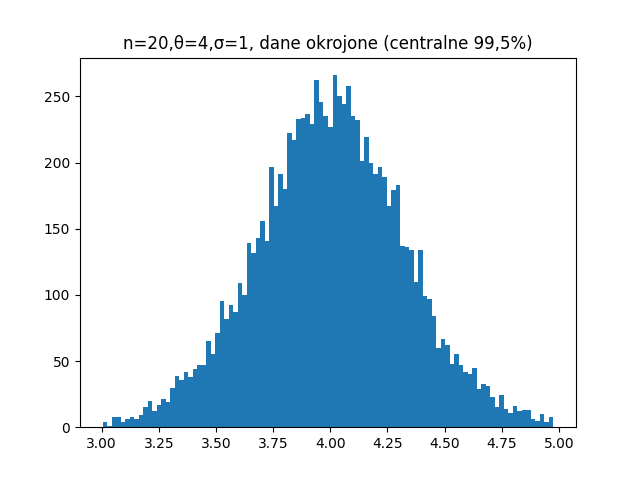
\includegraphics{Figure_1}\\
\end{center}



Obserwacje ogólne - eksperymenty dobrze pokazały jak wraz ze zwiększaniem próbki obciążenie estymatorów oraz ich błąd średniokwadratowy zbiegają do zera. Ciekawym okazał się przypadek wyznaczania numerycznego estymatorów największej wiarygodności dla zmiennych z rozkładu Cauchy'ego przy niewielkiej próbce, gdyż wymagał użycia bardziej wysublimowanych metod.

\end{document}
